\documentclass{ctexart}
\usepackage{tikz}
\usepackage{graphicx}

\begin{document}


\begin{figure}[htbp]
    \centering
    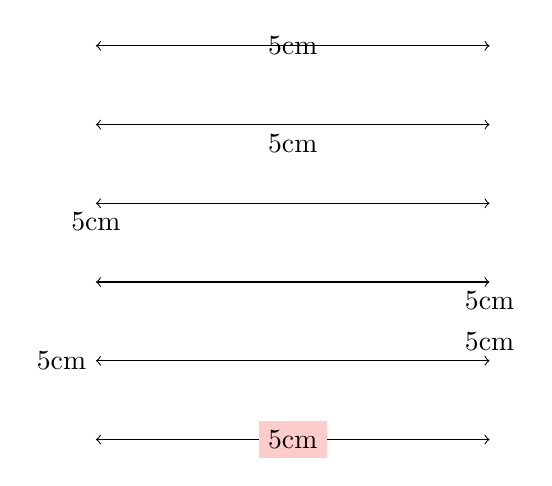
\begin{tikzpicture}
        \draw[<->] (0,1) -- node {5cm} (5,1);
        \draw[<->] (0,0) -- node[below]{5cm}(5,0);
        \draw[<->] (0,-1)node[below]{5cm} -- (5,-1);
        \draw[<->] (0,-2) -- (5,-2)node[below]{5cm};
        \draw[<->] (0,-3)node[left]{5cm} -- (5,-3)node[above]{5cm};
        \draw[<->] (0,-4) -- node[fill=red!20!white]{5cm}(5,-4);    % 百分之20的红色,百分之 80的白色 调用到xcolor包的时候都可以使用这种方式
    \end{tikzpicture}
    \caption{<caption>}
\end{figure}

\begin{figure}[htbp]
    \centering
    \begin{tikzpicture}[>=latex]
        \draw[->](-1,0) -- (4,0)node[right]{$x$};
        \draw[->](0,-1) -- (0,4)node[right]{$y$};
        \draw (0,2)node[left]{$N$} -- (2,2)node[right]{$P(x,y)$} -- (2,0)node[below]{$M$};

        \node at (-.2,-.2){$O$};
        \draw (0,1)node[left]{$1$} -- (.1,1);
        \draw (1,0)node[below]{$1$} -- (1,.1);
    \end{tikzpicture}
    \caption{}
\end{figure}

\begin{figure}[htbp]
    \centering
    \begin{tikzpicture}[>=latex]
        \draw[->](-1,0) -- (4,0)node[right]{$x$};
        \draw[->](0,-1) -- (0,4)node[right]{$y$};
        % \draw (0,2)node[left]{$N$} -- (2,2)node[right]{$P(x,y)$} -- (2,0)node[below]{$M$};

        \node at (-.2,-.2){$O$};
        % \draw (0,1)node[left]{$1$} -- (.1,1);
        % \draw (0,2)node[left]{$2$} -- (.1,2);
        % \draw (0,3)node[left]{$3$} -- (.1,3);
        \foreach \x in {1,2,...,6}
        {
            \draw (0,\x*0.5)node[left]{$\x$} -- (.1,\x*0.5);
            \draw (\x*0.5,0)node[below]{$\x$} -- (\x*0.5,.1);
        }
    \end{tikzpicture}
    \caption{}
\end{figure}

\begin{figure}[htbp]
    \centering
    \begin{tikzpicture}[>=latex,scale=.5]   % 只针对图进行缩放,不对文字进行缩放
        \draw[->](-5,0) -- (5,0)node[right]{$x$};
        \draw[->](0,-5) -- (0,5)node[right]{$y$};

        \node at (-.5,-.5){$O$};

    \end{tikzpicture}
    \caption{}
\end{figure}

\begin{figure}[htbp]
    \centering
    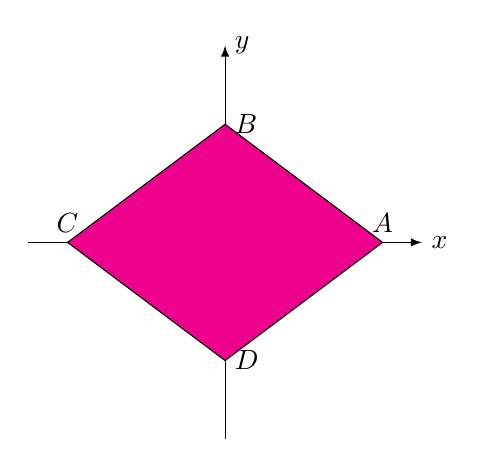
\begin{tikzpicture}[>=latex,scale=.5]   % 只针对图进行缩放,不对文字进行缩放
        \draw[->](-5,0) -- (5,0)node[right]{$x$};
        \draw[->](0,-5) -- (0,5)node[right]{$y$};

        \node at (-.5,-.5){$O$};

        \draw[fill=magenta] (-4,0)node[above]{$C$} -- (0,3)node[right]{$B$} -- (4,0)node[above]{$A$} -- (0,-3)node[right]{$D$} -- (-4,0) ;
    \end{tikzpicture}
    \caption{颜色填充}
\end{figure}

\begin{figure}[htbp]
    \centering
    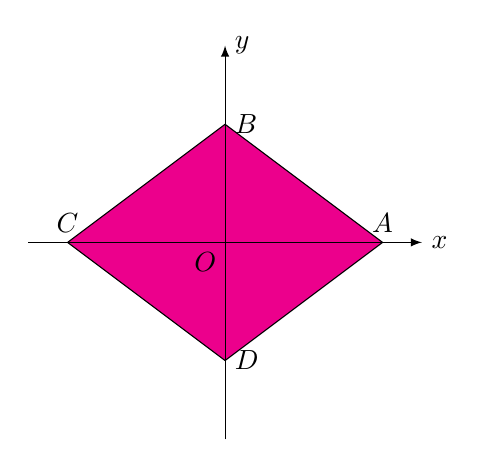
\begin{tikzpicture}[>=latex,scale=.5]   % 只针对图进行缩放,不对文字进行缩放
        
        \draw[fill=magenta] (-4,0)node[above]{$C$} -- (0,3)node[right]{$B$} -- (4,0)node[above]{$A$} -- (0,-3)node[right]{$D$} -- (-4,0) ;

        \draw[->](-5,0) -- (5,0)node[right]{$x$};
        \draw[->](0,-5) -- (0,5)node[right]{$y$};

        \node at (-.5,-.5){$O$};

    \end{tikzpicture}
    \caption{颜色填充}
\end{figure}

\begin{figure}[htbp]
    \centering
    
\begin{tikzpicture}[>=latex]   % 只针对图进行缩放,不对文字进行缩放
        
        \draw[fill=cyan] (0,0) rectangle (4,3);

    \end{tikzpicture}
    \caption{颜色填充}
\end{figure}

\begin{figure}[htbp]
    \centering
    
\begin{tikzpicture}[>=latex]  
        
        \fill[cyan] (0,0) rectangle (4,3);

    \end{tikzpicture}
    \caption{颜色填充}
\end{figure}

\begin{figure}[htbp]
    \centering
    
\begin{tikzpicture}[>=latex]  
        
        \fill[cyan,draw=black] (0,0) rectangle (4,3);

    \end{tikzpicture}
    \caption{颜色填充}
\end{figure}

\begin{figure}[htbp]
    \centering
    
\begin{tikzpicture}[>=latex]  
        
        \draw[fill=cyan] (0,0) circle (1.5) ;

    \end{tikzpicture}
    \caption{圆形}
\end{figure}

\begin{figure}[htbp]
    \centering
    \begin{tikzpicture}[>=latex]   
        
       \draw (0,0) -- (4,0);
    %    \draw (0,0) -- (4,4);
        \draw (0,0) -- (45:4);  % 极坐标表示
        \draw[->] (2,0) arc (0:45:2);

    \end{tikzpicture}
    \caption{圆弧}
\end{figure}

\begin{figure}[htbp]
    \centering
    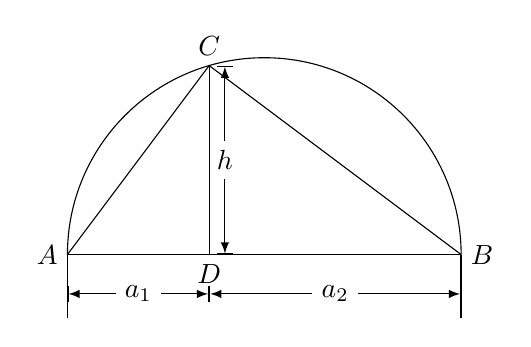
\begin{tikzpicture}[>=latex]   
        
        \draw (0,0)node[left]{$A$} -- (5,0)node[right]{$B$};
        \draw (0,0) arc (180:0:2.5);

        \draw (0,0) -- (1.8,2.4) -- (5,0) ;
        \draw[|<->|](0,-.5) --node[fill=white]{$a_1$} (1.8,-.5) ;
        \draw[|<->|](5,-.5) --node[fill=white]{$a_2$} (1.8,-.5) ;
        \draw (0,0) -- (0,-.8) ;
        \draw[thick] (5,0) -- (5,-.8) ;

        \draw[|<->|](2,2.4) --node[fill=white]{$h$} (2,0) ;
        \draw (1.8,2.4)node[above]{$C$} -- (1.8,0)node[below]{$D$} ;
    \end{tikzpicture}
    \caption{练习1}
\end{figure}

\begin{figure}[htbp]
    \centering
    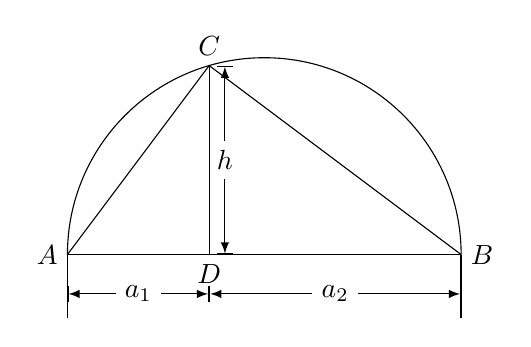
\begin{tikzpicture}[>=latex]   
        
        \draw (0,0)node[left]{$A$} -- (5,0)node[right]{$B$};
        \draw (0,0) arc (180:0:2.5);

        \draw (0,0) -- (1.8,2.4) -- (5,0) ;
        \draw[|<->|](0,-.5) --node[fill=white]{$a_1$} (1.8,-.5) ;
        \draw[|<->|](5,-.5) --node[fill=white]{$a_2$} (1.8,-.5) ;
        \draw (0,0) -- (0,-.8) ;
        \draw[thick] (5,0) -- (5,-.8) ;

        \draw[|<->|](2,2.4) --node[fill=white]{$h$} (2,0) ;
        \draw (1.8,2.4)node[above]{$C$} -- (1.8,0)node[below]{$D$} ;
    \end{tikzpicture}
    \caption{练习2}
\end{figure}
\end{document}